将地暖简化为第二类边界条件,即:
\begin{equation}
    -k\frac{\partial T}{\partial x}\big|_{x=L} = q
\end{equation}

式中q为地暖单位面积的放热量,为了方便计算,将上式写作:
\begin{equation}
    T_{x+dx} = T_x -\frac{q}{k}dx
\end{equation}

房间内温度分布如下图所示:
\begin{figure}[h]
    \centering
    \subfigure[主视图]{
    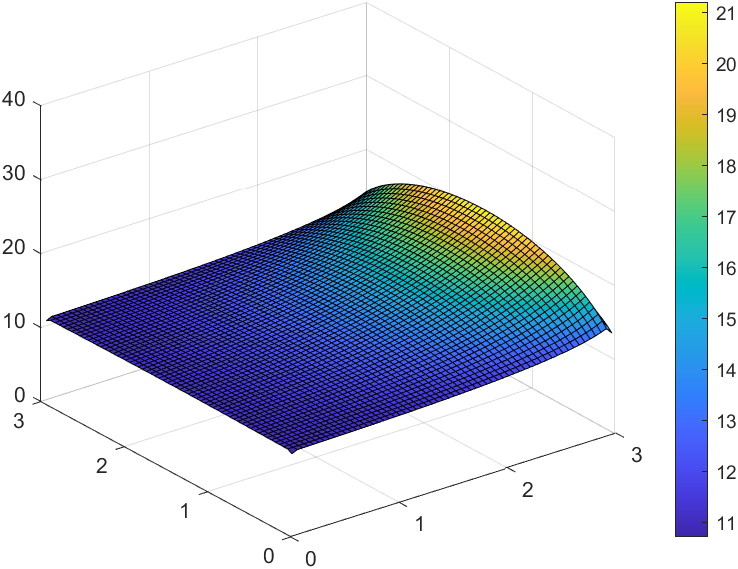
\includegraphics[width = 5.5cm]{figures/地暖主视.png}
    }\qquad
    \subfigure[俯视图]{
    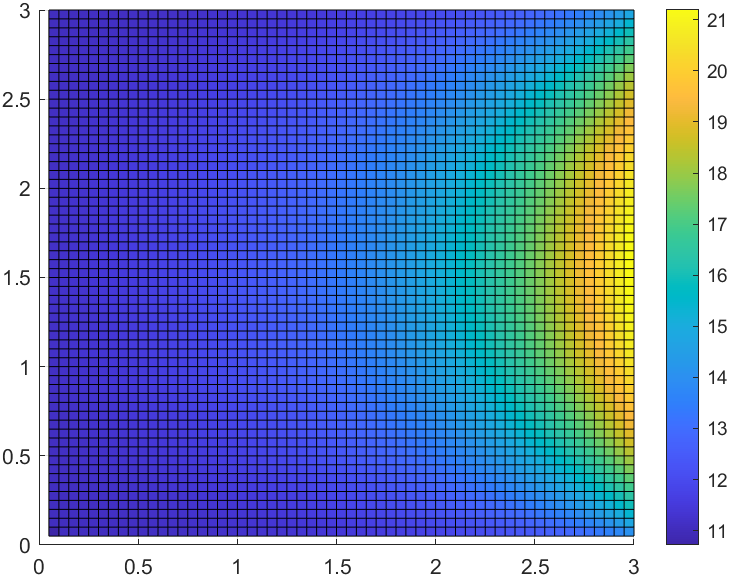
\includegraphics[width = 5.5cm]{figures/地暖俯视.png}
    }
    \caption{隔壁房间开地暖时的温度分布}
    \label{fig:dinuan}
\end{figure}

房间的平均温度为14℃,但是靠近地暖部分的温度较高。出现该现象的原因是地暖模型被过度简化,与现实中的地暖功能产生较大的偏差。因此还是使用开暖气时的隔壁房间平均温度作为待测房间的边界条件,同时考虑待测房间楼上开地暖时对于待测房间温度分布的影响。